%\section{Prediction Evaluation}
Recall from Section 2.4 that a receiver operating characteristic (ROC) curve is a metric for the ability of a classifier to discern between classes, where a larger area under the curve indicates better predictive performance. The y-axis is the true positive rate (sensitivity) and the x-axis is the false positive rate (1 - specificity). In this chapter, we discuss the changing predictive ability of our classifier as it went through various iterations visualized through ROC curves on four distinct validation sets.

For each of the below curves generated using our ensemble method, the threshold was the required percent of random forests in the ensemble to flag a contest as a positive for it to be labeled as a positive. (Once again, a flagged contest is one that will not fill to its target entries within the time that it is open to entries). Since our ensemble used 20 forests, each ROC was made from 20 threshold values. A ROC curve representing an optimal algorithm will flag every True Positive (TP) contest without flagging a single False Positive (FP). It is nearly impossible to create an algorithm with perfect sensitivity and specificity, so our goal was simply to maximize the area below the ROC curve. 
In the following graphics, many of the ROC curves are rainbow colored. This coloring is to help identify the threshold used to produce the indicated TP and FP rate pair.

\pagebreak

\section{Header Data Results}

\begin{figure}[h]
\centering
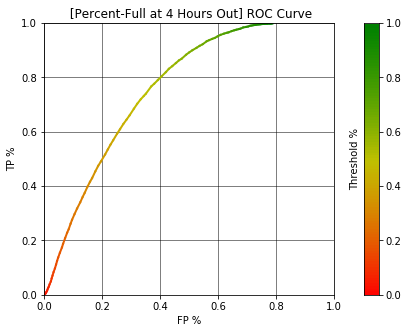
\includegraphics[width=10cm]{body/results/Graphs/JustMeta/1.Baseline/index.png}
\caption{ROC generated ROC generated using a threshold of percent filled at the ``4 Hour Out'' point. This represents an initial baseline estimation we needed to outperform.}
\label{fig:baseline}
\end{figure}

To ensure we weren't over-complicating our approach, our started by generating a simple baseline ROC curve. Figure \ref{fig:baseline} was generated for this purpose by moving the threshold through the column, ``Percent Full at 4 Hours Out''. At a threshold of 50\%, any contest which was less than 50\% full at the Time Series data point 4 hours before contest start was flagged as a positive. At that threshold, approximately 80\% of True Positives are flagged with only 40\% of False Positives flagged. This visual is a good way of showing the data-set is inherently highly imbalanced as it would seem we can achieve a decent prediction by simply evaluating each contest at the ``4 Hour Out'' mark with no need for a complicated prediction.
%it would be dope if you could actually put the points on the graph for your example but don't worry too much for this draft

\begin{figure}[h]
\centering
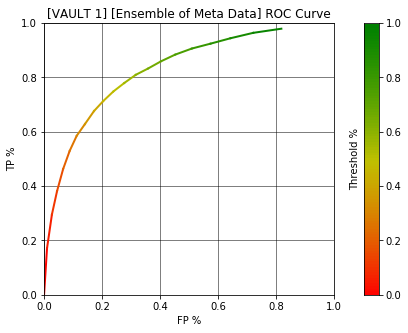
\includegraphics[width=8cm]{body/results/Graphs/JustMeta/2.MetaEnsemble/v1.png}
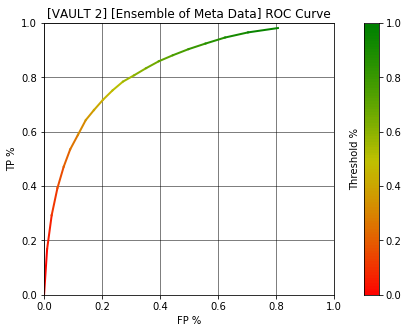
\includegraphics[width=8cm]{body/results/Graphs/JustMeta/2.MetaEnsemble/v2.png}
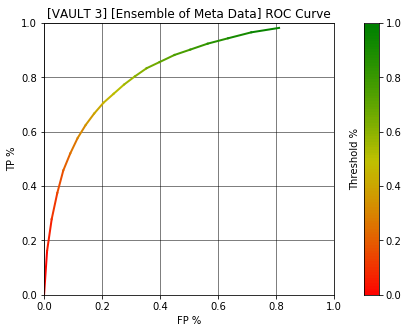
\includegraphics[width=8cm]{body/results/Graphs/JustMeta/2.MetaEnsemble/v3.png}
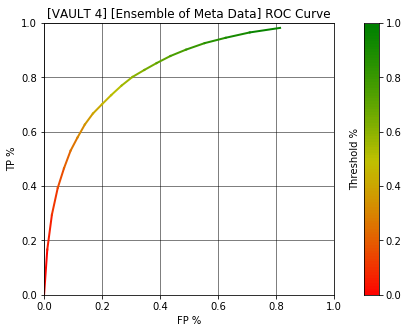
\includegraphics[width=8cm]{body/results/Graphs/JustMeta/2.MetaEnsemble/v4.png}
\caption{ROCs generated based on our ensemble of random forests using only processed Header data. Top Left: Validation set 1. Top Right: Validation set 2. Bottom Left: Validation set 3. Bottom Right: Validation set 4.}
\label{fig:metaonly}
\end{figure}

\pagebreak

Figure \ref{fig:metaonly} was generated using processed Header data in our ensemble of 20 Random Forest Classifiers (RFC). At a threshold of 50\%, approximately 80\% of True Positives are flagged with only 30\% False Positives being flagged in all four validation sets. These ROC curves consistently have 10\% better specificity than that of Figure \ref{fig:baseline} at this same threshold. Figure \ref{fig:metacomp} shows a direct comparison between the baseline curve and the curve from predicting using an ensemble of processed Header data for each validation set.

\pagebreak

\begin{figure}[h]
\centering
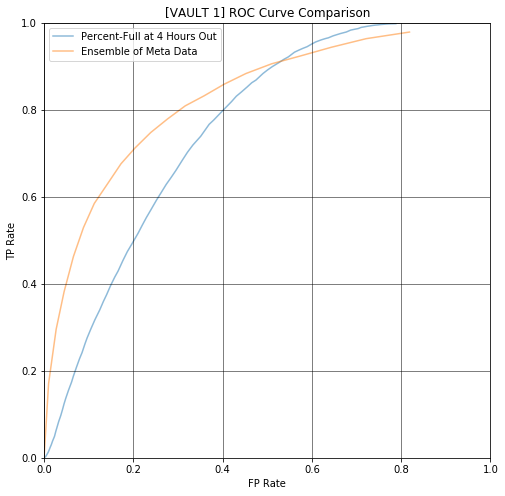
\includegraphics[width=8cm]{body/results/Graphs/JustMeta/3.Compare/v1.png}
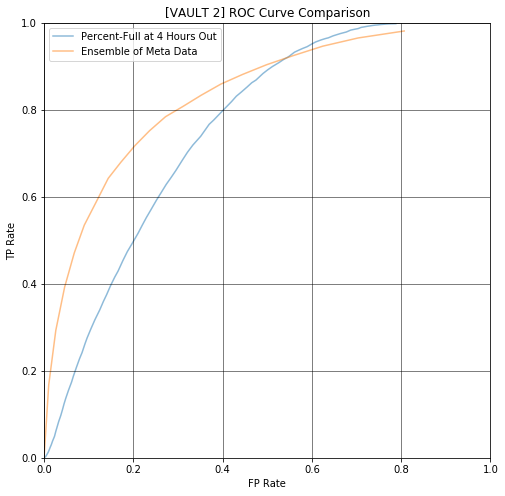
\includegraphics[width=8cm]{body/results/Graphs/JustMeta/3.Compare/v2.png}
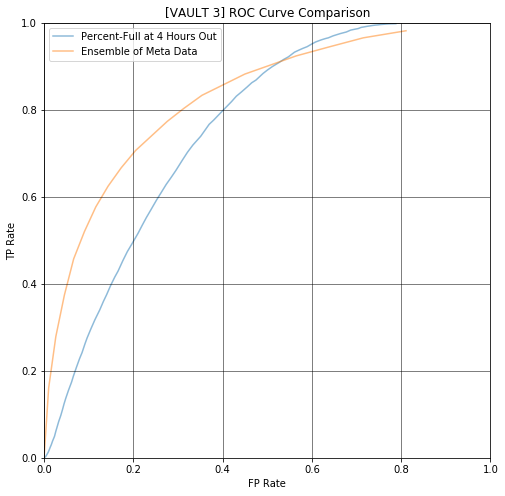
\includegraphics[width=8cm]{body/results/Graphs/JustMeta/3.Compare/v3.png}
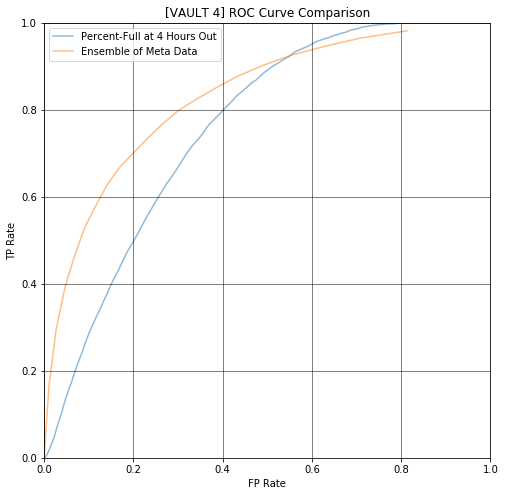
\includegraphics[width=8cm]{body/results/Graphs/JustMeta/3.Compare/v4.png}
\caption{Comparison of ROCs generated based on our ensemble of random forests using only processed Header data againt the baseline. Top Left: Validation set 1. Top Right: Validation set 2. Bottom Left: Validation set 3. Bottom Right: Validation set 4.}
\label{fig:metacomp}
\end{figure}

Figures \ref{fig:metaonly} and \ref{fig:metacomp} indicate that using an ensemble of Header data is useful for classifying contests. However, this does not yet include any of the Time Series Data.  


